\documentclass[a4paper, 12pt]{article}
\usepackage[utf8]{inputenc}
\usepackage{amsmath}
\usepackage{tikz, pgfplots, pgfplotstable}
\usetikzlibrary{positioning}
\pgfplotsset{compat=1.18}

\begin{document}

\section{Graphs of Different Equations: 2D plots}
\subsection{Graph of $x^2$}
\begin{figure}[!ht]
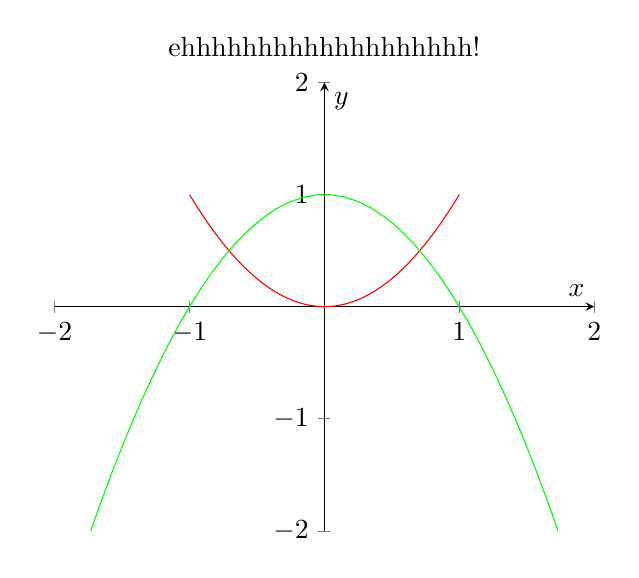
\begin{tikzpicture}
	\begin{axis}[
		xmin=-2, xmax=2, ymin=-2, ymax=2,
		axis lines=middle,
		xlabel=$x$,
		ylabel=$y$,
		title={ehhhhhhhhhhhhhhhhhhh!},
		]
		\addplot[red, samples=100, domain=-1:1]{x^2};
		\addplot[green, samples=100]{1-x^2};
	\end{axis}
\end{tikzpicture}
\end{figure}

\subsection{Sine-Cosine Graph $(Sin\theta, Cos\theta)$}
\begin{figure}[!ht]
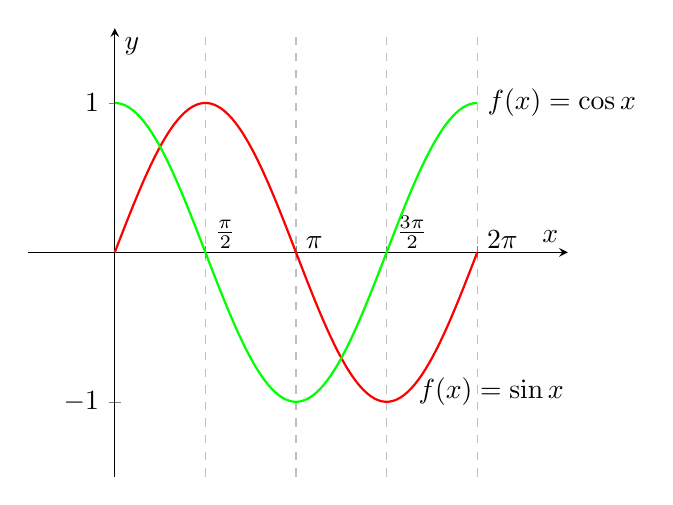
\begin{tikzpicture}
	\begin{axis}[
		clip=false,
		xmin=-1.5, xmax=2.5*pi,
		ymin=-1.5, ymax=1.5,
		axis lines=middle,
		xlabel=$x$, ylabel=$y$,
		xtick={pi/2, pi, 3*pi/2, 2*pi},
		xticklabels={$\frac{\pi}{2}$, $\pi$, $\frac{3\pi}{2}$, $2\pi$},
		xticklabel style={anchor=south west},
		xmajorgrids=true,
		grid style=dashed
		]
		\addplot[red, thick, samples=100, domain=0:2*pi]{sin(deg(x))} node[black, right, pos=0.8]{$f(x)=\sin x$};
		\addplot[green, thick, samples=100, domain=0:2*pi]{cos(deg(x))} node[black, right, pos=1]{$f(x)=\cos x$};
	\end{axis}
\end{tikzpicture}
\end{figure}

\newpage
\section{Different Indicator for different data}
\begin{figure} [!ht]
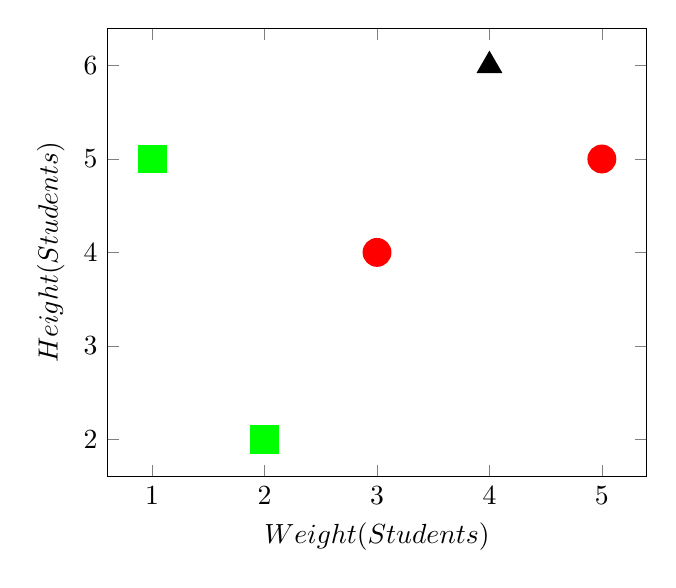
\begin{tikzpicture}
  \begin{axis}[
  	xlabel=$Weight(Students)$, 
  	ylabel=$Height(Students)$,
  	scatter/classes={
  			a={mark=square*, color=green},
  			b={mark=*, color=red},
  			c={mark=triangle*, color=black}	
  }
  ]
  	\addplot[
  		color=green,
  		only marks,
  		mark size=5px,
  		scatter,
  		scatter src=explicit symbolic,
  	] 
  		coordinates {
  			(2, 2) [a]
  			(3, 4) [b]
  			(1, 5) [a]
  			(4, 6) [c]
  			(5, 5) [b]
  		};
  	
  \end{axis}
\end{tikzpicture}
	\caption{Something that doesn't exist \label{fig:smthg}}
\end{figure}


\section{Graph of $Sin\theta$ and $Cos\theta$}
\
\begin{figure} [!ht]
	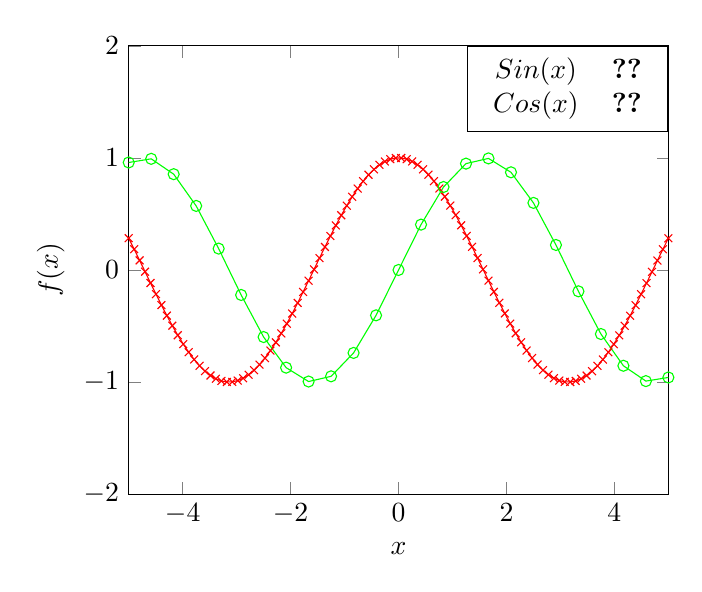
\begin{tikzpicture}
		\begin{axis}[
			name=plot,
			ymin=-2, ymax=2,
			xmin=-5, xmax=5,
			xlabel=$x$, 
			ylabel=$f(x)$,
		]
			\addplot[red, mark=x, samples=100] {cos(deg(x))}; \label{cosGraph}
			\addplot[green, mark=o] {sin(deg(x))}; \label{sinGraph}			
		\end{axis}
		
		\node[anchor=north east, draw=black, fill=white] at (plot.north east) {
			\begin{tabular}{c c}
				$Sin(x)$ & \ref{sinGraph}  \\
				$Cos(x)$ & \ref{cosGraph}
			\end{tabular}};
	\end{tikzpicture}
	\caption{Data from External \label{fig:ExtData}}
\end{figure}

\section{Trending Graph Comparison}
\begin{figure}[!ht]
	\centering
	\begin{tikzpicture}
		\begin{axis}[
		xlabel=Trend,
		ylabel=Data,
		legend entries={plot 1, plot 2, plot 3},
		reverse legend,
		legend pos=outer north east	
		]
		\addplot table [x=a, y=plot 1, col sep=comma]{mydata.csv};
		\addplot table [x=a, y=plot 2, col sep=comma]{mydata.csv};
		\addplot table [x=a, y=plot 3, col sep=comma]{mydata.csv};
		\end{axis}
	\end{tikzpicture}
	\caption{Trending graph comparison}
\end{figure}

\newpage
\section{Medium Graph 01: Economist Corbyn}
\subsection{Y-bar plotting}
\begin{figure}[!ht]
	\centering
	\begin{tikzpicture}
		\pgfplotstableread[col sep=comma]{EconomistCorbyn.csv}\corbynData
		\begin{axis}[
		ybar,
		width=12cm, height=8cm,
		bar width=1cm,
		xlabel=$Name Of The Pages$,
		ylabel=${Average likes per post (2016)}$,
		xtick=data,
		xticklabels from table={\corbynData}{Page},
		xticklabel style={rotate=90, anchor=east},
		nodes near coords,
		nodes near coords align={vertical},
		]
		\addplot table [x expr=\coordindex, y=Average number of likes per Facebook post 2016]{\corbynData};	
		\end{axis}
	\end{tikzpicture}
\end{figure}
\newpage
\subsection{X-bar plotting}
\begin{figure}[!ht]
	\begin{tikzpicture}
	\pgfplotstableread[col sep=comma]{EconomistCorbyn.csv}\corbynData
	\begin{axis}[
		xbar,
		width=12cm, height=8cm,
		bar width=0.8cm,
		ylabel=$Name Of The Pages$,
		xlabel=${Average Likes Per Post (2016)}$,
		ytick=data,
		yticklabels from table={\corbynData}{Page},
		yticklabel style={rotate=0, anchor=east},
		nodes near coords,
		nodes near coords align={horizontal},
		]
		\addplot table [y expr=\coordindex, x=Average number of likes per Facebook post 2016]{\corbynData};
	\end{axis}
	\end{tikzpicture}
\end{figure}
\end{document}
